\chapter{इलेक्ट्रॉनिकी: पुनर्भरण, दोलित्र और संकेत-ग्रहण}\label{ch:b2:feedback-oscillators}

कोई माइक्रोफ़ोन उस ध्वनिविस्तारक के बहुत पास ले जाइए जिसे वह चलाता है, और
भवन किसी चीख़ से भर जाता है: प्रवर्धक स्वयं को सुनने लगता है, और नन्हा-सा
रव किसी एक विशेष स्वर पर चीख़ बन जाता है। साध लिया जाए तो वही पाश हर
घड़ी, रेडियो और स्वर-संश्लेषक का हृदय है --- अर्थात् कोई \emph{दोलित्र},
जो लब्धि और छन्नी के सिवा कुछ भी न लेकर ज्यावक्र बना देता है। वर्ष 1 के
खंड ने संक्रियात्मक प्रवर्धक से प्रवर्धक, छन्नियाँ और तुलनित्र बनाए थे;
यह अध्याय उनके चारों ओर का पाश बंद करता है, पूछता है कि कोई पाश कब स्थायी
रहता है और कब दोलन करता है, दो दोलित्र बनाता है --- एक ज्यावक्रीय, एक
वर्गाकार --- और फिर उन दो संक्रियाओं की ओर मुड़ता है जिनसे कोई नापा गया
संकेत संगणक तक पहुँचता है: उसका \emph{प्रतिचयन}, और
\emph{\omterm{prop:b2:feedback-oscillators:lockin}{तुल्यकालिक संसूचन}} से उसे रव में से खींच लेना।

\begin{omfigure}
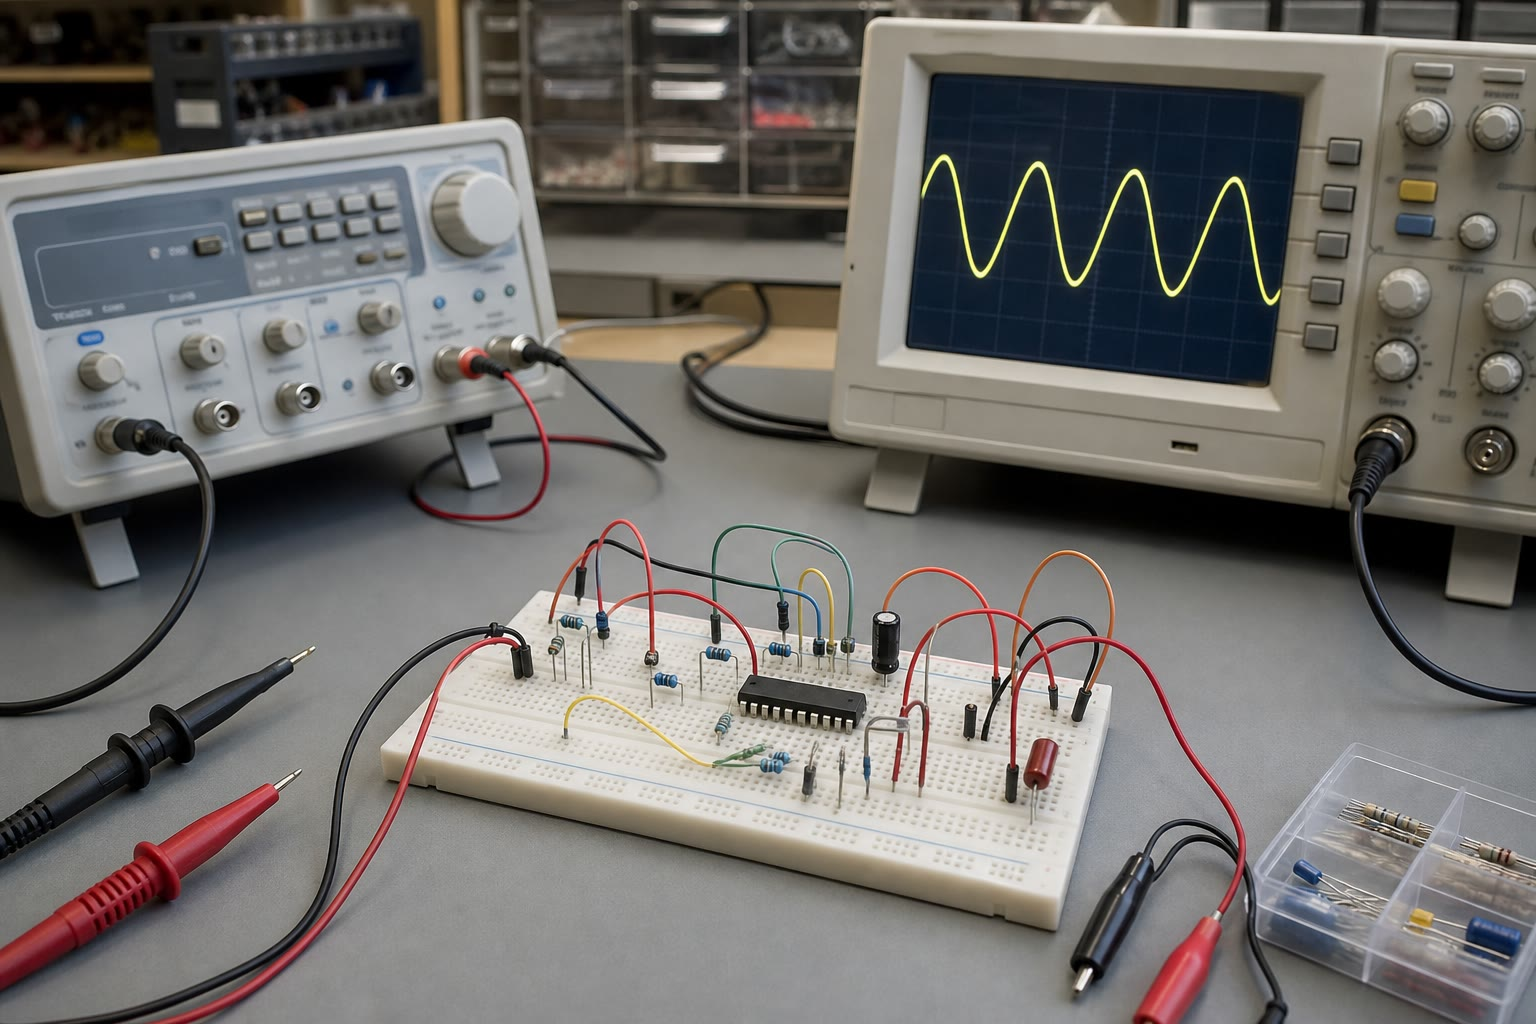
\includegraphics[width=0.58\linewidth]{images/book4/ai/b4-09-electronics-bench-oscillator.jpg}

{\small कोई ब्रेडबोर्ड, कोई फलन जनित्र और कोई दोलनदर्शी: वही मेज़ जिस पर पुनर्भरण-पाश बंद किया जाता है --- और जिस पर, प्रवर्धक के गाने लगते ही, यह पता चलता है कि वह दोलित्र बन चुका है।}
\end{omfigure}


\section{पुनर्भरण और स्थायित्व}

\begin{definition}[बंद पाश; पाश-लब्धि]\label{def:b2:feedback-oscillators:loop}
\index{पुनर्भरण}\index{पाश-लब्धि}\index{बंद-पाश अंतरण फलन}
$\underline A(\jmath\omega)$ अंतरण फलन का कोई प्रवर्धक
निवेश $\underline e$ के साथ अंश $\underline\beta(\jmath\omega)\,\underline s$ भी पाता
है, जो उसके अपने निर्गम $\underline s$ का है (धनात्मक पुनर्भरण;
ऋणात्मक पुनर्भरण के लिए $\beta$ का चिह्न बदल दीजिए)। \emph{बंद-पाश}
अंतरण फलन और \emph{पाश-लब्धि} ये हैं:
\[
\underline H = \frac{\underline s}{\underline e} = \frac{\underline A}{1 - \underline A\,\underline\beta} ,
\qquad \underline T = \underline A\,\underline\beta .
\]
\end{definition}

\begin{theorem}[किसी रैखिक पाश का स्थायित्व; दोलन का प्रतिबंध]\label{thm:b2:feedback-oscillators:stability}
\index{स्थायित्व (रैखिक निकाय)}\index{बार्कहाउज़ेन प्रतिबंध}\index{अभिलक्षणिक समीकरण}
$\jmath\omega$ की जगह सम्मिश्र चर $p$ रखने पर पाश का मुक्त विकास
उसके \emph{\omterm{thm:b2:feedback-oscillators:stability}{अभिलक्षणिक समीकरण}}
$1 - \underline A(p)\underline\beta(p) = 0$ के मूलों ($\underline H$ के ध्रुवों) से चलता है: हर मूल
$p_i$ एक विधा $\eu^{p_it}$ देता है। पाश तब \emph{स्थायी} है जब सब
मूलों के वास्तविक भाग ऋणात्मक हों (तब हर विधा मर जाती है); और वह
बढ़ते आयाम के साथ \emph{दोलन} करता है जब किसी मूल का वास्तविक भाग
धनात्मक हो। सीमा --- अर्थात् शुद्ध काल्पनिक मूलों का कोई युग्म $\pm\jmath
\omega_0$, अर्थात् कोई टिकाऊ ज्यावक्र --- तब आती है जब
\[
\underline A(\jmath\omega_0)\,\underline\beta(\jmath\omega_0) = 1
\]
हो (\emph{\omterm{thm:b2:feedback-oscillators:stability}{बार्कहाउज़ेन प्रतिबंध}}: $\omega_0$ पर \omterm{def:b2:feedback-oscillators:loop}{पाश-लब्धि} का मापांक एक और कला
शून्य)। किसी द्वितीय-कोटि हर $ap^2 + bp + c$ के लिए
पाश तभी और केवल तभी स्थायी है जब $a$, $b$, $c$ के चिह्न एक हों।
\end{theorem}

\begin{proof}
पाश का अवकल समीकरण $\underline s(1 -
\underline A\underline\beta) = \underline A\underline e$ से मिलता है, यदि $\jmath\omega$ की हर घात को
समय-अवकलज पढ़ा जाए; और उसके समांगी हल $\eu^{p_it}$ हैं,
जहाँ $p_i$ बहुपद के मूल हैं। बढ़ना या घटना
$\operatorname{Re}p_i$ के चिह्न से चलता है; और किसी द्वितीय-कोटि बहुपद के मूलों के
वास्तविक भाग ठीक तब ऋणात्मक होते हैं जब गुणांकों का चिह्न एक हो
(उनका योग $-b/a$ और गुणनफल $c/a$ है)। बार्कहाउज़ेन का प्रतिबंध
$p = \jmath\omega_0$ पर किसी मूल के होने का प्रतिबंध है।
\end{proof}

\begin{remark}[कोई दोलित्र कैसे चलता और रुकता है]\label{rem:b2:feedback-oscillators:start}
कोई दोलित्र इस तरह बनाया जाता है कि $\omega_0$ पर \omterm{def:b2:feedback-oscillators:loop}{पाश-लब्धि} एक से कुछ
\emph{अधिक} हो: चालू होते समय जो रव होता है उसमें वह आवृत्ति भी होती है,
जो चरघातांकी रूप से बढ़ती है जबकि बाक़ी सब मर जाती हैं। तब रैखिक सिद्धांत
अनंत आयाम बताता है; पर वास्तव में कोई \emph{अरैखिकता} ---
प्रवर्धक की संतृप्ति, या कोई जान-बूझकर लगाया अरैखिक
अवयव --- आयाम बढ़ते ही प्रभावी लब्धि घटा देती है, जब तक
\omterm{def:b2:feedback-oscillators:loop}{पाश-लब्धि} का औसत ठीक एक न हो जाए: और तब आयाम ठहर जाता है। इस तरह हर असली
दोलित्र आवृत्ति के लिए रैखिक पाश है और आयाम के लिए अरैखिक;
और सीमन जितना कोमल, ज्यावक्र उतना ही शुद्ध।
\end{remark}

\section{वीन-सेतु दोलित्र}

\begin{proposition}[वीन-सेतु दोलित्र]\label{prop:b2:feedback-oscillators:wien}
\index{वीन-सेतु दोलित्र}\index{वीन जाल}
$K = 1 + R_2/R_1$ लब्धि की अव्युत्क्रमी रचना में लगा कोई संक्रियात्मक प्रवर्धक
अपना निर्गम \emph{\omterm{prop:b2:feedback-oscillators:wien}{वीन जाल}} से होकर अपने $+$ निवेश पर लौटाता है:
अर्थात् $R$ और $C$ श्रेणी में, फिर $R$ और $C$ समांतर में भू से। इस
जाल का अंतरण फलन
\[
\underline\beta(\jmath\omega) = \frac1{3 + \jmath(RC\omega - 1/RC\omega)} ,
\]
है, जो वास्तविक और अधिकतम ($= 1/3$) होता है, $\omega_0 = 1/RC$ पर। \omterm{def:b2:feedback-oscillators:loop}{पाश-लब्धि} $K\underline\beta$
$\omega_0$ पर एक के बराबर तब होती है जब $K = 3$: और तब परिपथ इस आवृत्ति पर
ज्यावक्र टिकाए रखता है:
\[
f_0 = \frac1{2\pi RC} .
\]
वोल्टता $v$, जो $+$ निवेश पर है, इसका पालन करती है:
\[
\frac{\dd^2v}{\dd t^2} + \frac{3 - K}{RC}\,\frac{\dd v}{\dd t} + \frac{v}{R^2C^2} = 0 :
\]
अर्थात् $K < 3$ के लिए दोलन मर जाता है, और $K > 3$ के लिए वह $2RC/(K - 3)$
समय-नियतांक के साथ बढ़ता है (ऋणात्मक अवमंदन), जब तक संक्रियात्मक प्रवर्धक की
संतृप्ति उसे सीमित न कर दे।
\end{proposition}

\begin{proof}
वोल्टता-विभाजक: श्रेणी शाखा $Z_s = R + 1/\jmath C\omega$, समांतर
शाखा $Z_p = R/(1 + \jmath RC\omega)$; और $\underline\beta = Z_p/(Z_s + Z_p)$, जो
दिए गए रूप में सरल हो जाता है। पाश: $\underline v = \underline\beta K\underline v$, अर्थात्
$[3 + \jmath(RC\omega - 1/RC\omega)]\underline v = K\underline v$; अब $\jmath\omega RC$ से गुणा कीजिए
और $\jmath\omega \to \dd/\dd t$ पढ़िए: $R^2C^2\ddot v + (3 - K)RC\dot v + v = 0$।
इसका अवमंदन-गुणांक $K = 3$ पर चिह्न बदल देता है।
\end{proof}

\begin{omfigure}
\begin{tikzpicture}[font=\small, x=1cm, y=1cm, >=Stealth, scale=0.9, every node/.style={transform shape}]
  \begin{scope}
    \node[draw, thick, minimum width=1.4cm, minimum height=0.8cm] (A) at (0,0) {$\underline A$};
    \node[draw, thick, minimum width=1.4cm, minimum height=0.8cm] (B) at (0,-1.7) {$\underline\beta$};
    \draw[thick] (-2.3,0) circle (0.2); \node at (-2.3,0) {$+$};
    \draw[thick, ->] (-3.2,0) -- (-2.5,0) node[above, pos=0.3, font=\footnotesize] {$\underline e$};
    \draw[thick, ->] (-2.1,0) -- (A.west);
    \draw[thick, ->] (A.east) -- (2.0,0) node[above, pos=0.6, font=\footnotesize] {$\underline s$};
    \draw[thick] (1.4,0) -- (1.4,-1.7) -- (B.east);
    \draw[thick, ->] (B.west) -- (-2.3,-1.7) -- (-2.3,-0.2);
    \node[font=\footnotesize] at (-0.3,-2.7) {$\underline H = \dfrac{\underline A}{1 - \underline A\underline\beta}$};
  \end{scope}
\end{tikzpicture}
\hfill
\begin{tikzpicture}[font=\small, scale=0.78, every node/.style={transform shape}]
    \draw (0,0) node[op amp, noinv input down] (oa) {};
    % negative feedback: R2 from output to - input, R1 from - input to ground
    \coordinate (M) at ($(oa.-)+(-0.7,0)$);
    \draw (oa.-) -- (M);
    \draw (M) to[R, l_=$R_1$] ++(-1.6,0) node[ground, rotate=-90]{};
    \draw (M) -- ++(0,1.4) coordinate (T) to[R, l=$R_2$] (T -| oa.out) -- (oa.out);
    % Wien network: from output down, series C and R to node P, P to + input; P to ground via R and via C
    \coordinate (P) at (-3.4,-2.3);
    \draw (oa.out) -- ++(0.6,0) coordinate (O) -- (O |- P) to[C, l=$C$] ++(-1.6,0) to[R, l=$R$] (P);
    \draw (P) -- (P |- oa.+) -- (oa.+);
    \draw (P) to[R, l_=$R$] ++(0,-1.6) node[ground]{};
    \draw (P) -- ++(-1.1,0) coordinate (Q) to[C, l_=$C$] ++(0,-1.6) node[ground]{};
    \draw (O) to[short, -o] ++(0.5,0) node[right, font=\footnotesize] {$s$};
\end{tikzpicture}

{\small बाएँ: कोई पुनर्भरण-पाश --- निर्गम $\underline\beta$ से होकर
प्रवर्धक के निवेश पर लौटाया जाता है। दाएँ: \omterm{prop:b2:feedback-oscillators:wien}{वीन-सेतु
दोलित्र} --- $1 + R_2/R_1$ लब्धि का कोई अव्युत्क्रमी प्रवर्धक, जिसका
निर्गम उसके $+$ निवेश पर श्रेणी--समांतर $RC$ जाल से होकर लौटता है;
और लब्धि के 3 पर पहुँचते ही वह $1/2\pi RC$ पर दोलन करने लगता है।}
\end{omfigure}

\begin{example}[एक \qty{1}{kHz} स्रोत]\label{ex:b2:feedback-oscillators:wiennumbers}
$R = \qty{15.9}{k\ohm}$, $C = \qty{10}{nF}$: $f_0 = \qty{1.00}{kHz}$। $R_1 =
\qty{10}{k\ohm}$ और $R_2 = \qty{21}{k\ohm}$ लेकर $K = 3.1$: तब आयाम चालू होने के रव से
$\eu$ गुना बढ़ता है हर $2RC/0.1 = \qty{3.2}{ms}$ में, और कुछ दसियों
मिलीसेकंड में संतृप्ति तक पहुँच जाता है; और कटा हुआ ज्यावक्र तब
संनादियों से भरा होता है। $R_1$ की जगह कोई छोटा तापदीप्त बल्ब लगाइए, जिसका
प्रतिरोध गरम होते ही बढ़ता है, तो वह किसी मध्यम आयाम पर $K$ को ठीक $3$ तक
खींच लाता है: और तब $0.1\%$ से कम विरूपण का ज्यावक्र मिलता है ---
यही पहले प्रयोगशाला-संकेत जनित्रों का परिपथ था।
\end{example}

\section{शैथिल्य वाले तुलनित्र; अस्थायी बहुकंपित्र}

\begin{proposition}[शैथिल्य तुलनित्र]\label{prop:b2:feedback-oscillators:schmitt}
\index{शैथिल्य तुलनित्र}\index{श्मिट ट्रिगर}
\emph{धनात्मक} \omterm{def:b2:feedback-oscillators:loop}{पुनर्भरण} वाला कोई संक्रियात्मक प्रवर्धक --- जिसका निर्गम
$+$ निवेश पर किसी विभाजक $R_1$, $R_2$ से होकर जाता है (तब $+$ निवेश
$\beta s$ पर बैठता है, जहाँ $\beta = R_1/(R_1 + R_2)$, और संकेत $e$ $-$ निवेश पर लगाया जाता है)
--- का कोई स्थायी रैखिक व्यवहार नहीं होता: उसका निर्गम $+V_{\text{संतृप्त}}$ या
$-V_{\text{संतृप्त}}$ पर बैठता है और इस तरह पलटता है:
\begin{align*}
&\text{निर्गम } +V_{\text{संतृप्त}} \text{ से } -V_{\text{संतृप्त}} \text{ को, जब } e \text{ उस मान से ऊपर जाए जो है } +\beta V_{\text{संतृप्त}} ,\\
&\text{निर्गम } -V_{\text{संतृप्त}} \text{ से } +V_{\text{संतृप्त}} \text{ को, जब } e \text{ उस मान से नीचे जाए जो है } -\beta V_{\text{संतृप्त}} .
\end{align*}
दोनों देहलियाँ भिन्न हैं: \emph{शैथिल्य} $2\beta V_{\text{संतृप्त}}$ तुलनित्र को
उससे छोटे रव के प्रति अभेद्य बना देता है, और
$(e, s)$ तल में उसका चक्र दक्षिणावर्त चलता कोई आयत है।
\end{proposition}

\begin{proof}
$s = +V_{\text{संतृप्त}}$ पर $+$ निवेश $+\beta V_{\text{संतृप्त}}$ पर होता है; और निर्गम
तब तक धनात्मक रहता है जब तक $e < \beta V_{\text{संतृप्त}}$, और $e$ के उसे पार करते ही
पलट जाता है --- जिसके बाद $+$ निवेश $-\beta V_{\text{संतृप्त}}$ पर होता है, अतः $e$ को
उसे वापस पलटाने के लिए उससे नीचे गिरना पड़ता है। (रैखिक व्यवहार में धनात्मक
\omterm{def:b2:feedback-oscillators:loop}{पुनर्भरण} किसी भी विचलन को बढ़ा देता: वह अस्थायी है।)
\end{proof}

\begin{proposition}[अस्थायी बहुकंपित्र]\label{prop:b2:feedback-oscillators:astable}
\index{अस्थायी बहुकंपित्र}\index{शिथिलन दोलित्र}
\omterm{prop:b2:feedback-oscillators:schmitt}{शैथिल्य तुलनित्र} का निर्गम उसके अपने $-$ निवेश पर किसी $RC$ परिपथ से होकर
लौटाइए ($R$ $s$ से $-$ निवेश तक, और $C$ वहाँ से
भू तक)। संधारित्र $\pm V_{\text{संतृप्त}}$ की ओर आवेशित होता है और जब भी वह किसी
देहली पर पहुँचता है तुलनित्र को पलट देता है: अतः $s$ पर कोई वर्ग-तरंग, और
$C$ पर लगभग त्रिभुजाकार तरंग, जिसका आवर्तकाल
\[
T = 2RC\,\ln\frac{1 + \beta}{1 - \beta} .
\]
है। $\beta = 1/2$ के लिए $T = 2RC\ln3 \approx 2.2RC$। ऐसे \emph{\omterm{prop:b2:feedback-oscillators:astable}{शिथिलन
दोलित्र}} सूक्ष्म-नियंत्रकों की घड़ी चलाते हैं, संकेतक टिमटिमाते हैं और
फलन जनित्रों की त्रिभुज तथा वर्ग तरंगें बनाते हैं।
\end{proposition}

\begin{proof}
$s = +V_{\text{संतृप्त}}$ पर संधारित्र की वोल्टता $v_C$
$-\beta V_{\text{संतृप्त}}$ से $+V_{\text{संतृप्त}}$ की ओर $v_C = V_{\text{संतृप्त}} - (1 + \beta)
V_{\text{संतृप्त}}\eu^{-t/RC}$ के अनुसार जाती है, और $+\beta V_{\text{संतृप्त}}$ पर $RC\ln[(1 + \beta)
/(1 - \beta)]$ बाद पहुँचती है; तब तुलनित्र पलटता है और सममित अर्ध-चक्र चलता है।
\end{proof}

\begin{omfigure}
\begin{tikzpicture}
\begin{axis}[omaxis, axis x line=middle, axis y line=middle, width=5.6cm, height=4.6cm,
    xlabel={$e$}, ylabel={$s$}, xmin=-1.6, xmax=1.6, ymin=-1.5, ymax=1.5,
    xtick=\empty, ytick=\empty, clip=false]
  \node[font=\scriptsize, anchor=north] at (axis cs:-0.5,-1.55) {$-\beta V_{\text{संतृप्त}}$};
  \node[font=\scriptsize, anchor=north] at (axis cs:0.5,-1.55) {$\beta V_{\text{संतृप्त}}$};
  \node[font=\scriptsize, anchor=east] at (axis cs:-1.55,1) {$V_{\text{संतृप्त}}$};
  \node[font=\scriptsize, anchor=east] at (axis cs:-1.55,-1) {$-V_{\text{संतृप्त}}$};
  \draw[dotted] (axis cs:-0.5,0) -- (axis cs:-0.5,-1.5); \draw[dotted] (axis cs:0.5,0) -- (axis cs:0.5,-1.5);
  \addplot[omDef, very thick] coordinates {(-1.5,1) (0.5,1)};
  \addplot[omDef, very thick, ->] coordinates {(0.5,1) (0.5,-1)};
  \addplot[omDef, very thick] coordinates {(0.5,-1) (-0.5,-1)};
  \addplot[omDef, very thick, ->] coordinates {(-0.5,-1) (-0.5,1)};
  \addplot[omDef, very thick] coordinates {(-0.5,-1) (1.5,-1)};
\end{axis}
\end{tikzpicture}
\hfill
\begin{tikzpicture}
\begin{axis}[omaxis, axis x line=middle, axis y line=left, width=8.0cm, height=4.6cm,
    xlabel={$t$}, ylabel={}, xmin=0, xmax=4.4, ymin=-1.4, ymax=1.4, xtick=\empty, ytick={-1,-0.5,0.5,1},
    yticklabels={$-V_{\text{संतृप्त}}$, $-\beta V_{\text{संतृप्त}}$, $\beta V_{\text{संतृप्त}}$, $V_{\text{संतृप्त}}$}, tick label style={font=\scriptsize}, samples=60,
    xlabel style={at={(axis description cs:1.0,0.5)}, anchor=west},
    legend style={font=\scriptsize, at={(0.5,1.02)}, anchor=south, legend columns=2, draw=none, fill=none}]
  \addplot[omThm, thick] coordinates {(0,1) (1.1,1) (1.1,-1) (2.2,-1) (2.2,1) (3.3,1) (3.3,-1) (4.4,-1)};
  \addplot[omDef, thick, domain=0:1.1] {1-1.5*exp(-x)};
  \addplot[omDef, thick, domain=1.1:2.2] {-1+1.5*exp(-(x-1.1))};
  \addplot[omDef, thick, domain=2.2:3.3] {1-1.5*exp(-(x-2.2))};
  \addplot[omDef, thick, domain=3.3:4.4] {-1+1.5*exp(-(x-3.3))};
  \legend{$s$ (वर्ग), $v_C$}
\end{axis}
\end{tikzpicture}

{\small बाएँ: किसी \omterm{prop:b2:feedback-oscillators:schmitt}{शैथिल्य तुलनित्र} का चक्र --- दो देहलियाँ,
और दक्षिणावर्त चलता कोई आयत। दाएँ: \omterm{prop:b2:feedback-oscillators:astable}{अस्थायी बहुकंपित्र} ---
संधारित्र की वोल्टता देहलियों के बीच डोलती है और निर्गम
कोई वर्ग-तरंग होता है।}
\end{omfigure}

\section{किसी संकेत का प्रतिचयन}

\begin{theorem}[प्रतिचयन; नाइक्विस्ट--शैनन कसौटी]\label{thm:b2:feedback-oscillators:shannon}
\index{प्रतिचयन}\index{नाइक्विस्ट--शैनन कसौटी}\index{छद्मन}\index{छद्मन-रोधी छन्नी}
किसी संकेत का \emph{प्रतिचयन} तब होता है जब केवल उसके मान $s(nT_s)$
क्षणों $nT_s$ पर रखे जाएँ, और $f_s = 1/T_s$ \emph{प्रतिचयन दर} हो।
प्रतिचयित संकेत का वर्णक्रम $s$ के वर्णक्रम की वह पुनरावृत्ति है जो
$f_s$ के हर गुणज के चारों ओर बनती है। जिस संकेत का वर्णक्रम
$f_{\max}$ से नीचे सिमटा हो, उसे उसके प्रतिदर्शों से ठीक-ठीक फिर से बनाया
जा सकता है, तभी और केवल तभी जब
\[
f_s > 2f_{\max} ;
\]
हो; अन्यथा प्रतियाँ अतिव्यापी हो जाती हैं और $f > f_s/2$ का कोई घटक
\emph{छद्म} आवृत्ति $|f - nf_s|$ पर फिर उभर आता है (उस पूर्णांक $n$ के लिए जो
उसे $f_s/2$ से नीचे ले आए), जो किसी सच्चे नीची-आवृत्ति के घटक से
अभेद्य होता है। इसीलिए हर प्रतिचायक से पहले \emph{\omterm{thm:b2:feedback-oscillators:shannon}{छद्मन-रोधी छन्नी}}
रखी जाती है: कोई निम्न-पारक, जो $f_s/2$ से ऊपर का सब कुछ हटा दे।
\end{theorem}

\begin{proof}
प्रतिचयन का अर्थ है $s(t)$ को $T_s$ आवर्तकाल के सँकरे स्पंदों की किसी
आवर्ती रेल से गुणा करना, जिसकी फूरिये श्रेणी में सारे संनादी $nf_s$ होते हैं
(इस वर्ष का गणित-खंड); और $s$ को $\cos(2\pi nf_st)$ से गुणा करना
उसका वर्णक्रम $\pm nf_s$ से खिसका देता है --- यहीं से वे प्रतियाँ आती हैं। वे तभी और केवल तभी
अतिव्यापी नहीं होतीं जब $f_{\max} < f_s - f_{\max}$; और तब $f_s/2$ कटाव की कोई निम्न-पारक
मूल वर्णक्रम ठीक-ठीक वापस दे देती है (स्वीकृत)। छद्मन:
$\cos(2\pi ft)$ और $\cos(2\pi(f - nf_s)t)$ के प्रतिदर्श
$t = mT_s$ पर मिल जाते हैं, क्योंकि $2\pi nf_smT_s = 2\pi nm$।
\end{proof}

\begin{example}[गाड़ी के पहिये, सीडी और दोलनदर्शी]\label{ex:b2:feedback-oscillators:alias}
प्रति सेकंड $24$ चित्रों की कोई फ़िल्म संसार का प्रतिचयन \qty{24}{Hz} पर करती है: तब
$12$ तीलियों वाला कोई पहिया, जो प्रति सेकंड $2.1$ चक्कर लगाता हो, प्रति सेकंड
$25.2$ बार कोई तीली दिखाता है, अर्थात् $1.2$ ऊपर $f_s$ से --- अतः वह धीरे-धीरे
आगे घूमता लगता है, और प्रति सेकंड $1.9$ चक्कर से पीछे। कोई कॉम्पैक्ट डिस्क
\qty{20}{kHz} तक की ध्वनि लौटाने के लिए \qty{44.1}{kHz} पर प्रतिचयन करती है, और
$20$ तथा \qty{22}{kHz} के बीच खड़ी \omterm{thm:b2:feedback-oscillators:shannon}{छद्मन-रोधी छन्नी} रखती है। \qty{1}{MS/s} पर लगा कोई
अंकीय दोलनदर्शी \qty{999}{kHz} के ज्यावक्र को \qty{1}{kHz} का दिखाता है ---
अर्थात् अंकीय मापन का पहला जाल।
\end{example}

\begin{omfigure}
\begin{tikzpicture}
\begin{axis}[omaxis, axis x line=middle, axis y line=none, width=13.6cm, height=4.0cm,
    xmin=0, xmax=10, ymin=-1.4, ymax=1.5, xtick=\empty, samples=400, xlabel={$t$},
    xlabel style={at={(axis description cs:1.0,0.5)}, anchor=west},
    legend style={font=\scriptsize, at={(0.5,1.02)}, anchor=south, legend columns=3, draw=none, fill=none}]
  \addplot[omDef, thick, domain=0:10] {cos(deg(2*pi*0.9*x))};
  \addplot[omThm, thick, dashed, domain=0:10] {cos(deg(2*pi*0.1*x))};
  \addplot[only marks, mark=*, mark size=1.6pt, black, samples=11, domain=0:10] {cos(deg(2*pi*0.9*x))};
  \legend{$f = 0.9f_s$, $0.1f_s$ पर छद्म, प्रतिदर्श}
\end{axis}
\end{tikzpicture}

{\small छद्मन: $0.9f_s$ का कोई ज्यावक्र और $0.1f_s$ का कोई ज्यावक्र
उन्हीं प्रतिदर्शों से गुज़रते हैं; और एक बार प्रतिचयित हो जाने पर उन्हें अलग नहीं
किया जा सकता --- इसीलिए कसौटी $f_s > 2f_{\max}$।}
\end{omfigure}

\begin{remark}[क्वांटीकरण]\label{rem:b2:feedback-oscillators:quantization}
\index{क्वांटीकरण}\index{अनुरूप-से-अंकीय परिवर्तित्र}
\omterm{rem:b2:feedback-oscillators:quantization}{अनुरूप-से-अंकीय परिवर्तित्र} हर प्रतिदर्श को
$2^N$ स्तरों ($N$ बिट) में से एक तक पूर्णांकित भी कर देता है: और यह पूर्णांकन-त्रुटि, जो अधिक से अधिक आधा सोपान है,
$\Delta/\sqrt{12}$ वर्ग-माध्य-मूल के किसी रव की तरह काम करती है, जहाँ सोपान $\Delta$ है, तथा
गतिक परास (उस रव के सामने सबसे बड़ा ज्यावक्र) लगभग $6N + 2$ dB होता है ---
अर्थात् किसी सीडी के $16$ बिट के लिए \qty{98}{dB}, और किसी $12$-बिट
दोलनदर्शी के लिए \qty{74}{dB}। प्रतिचयन दर और विभेदन ही वे दो अंक हैं जो हर
अंकीयकारक के लेबल पर लिखे रहते हैं।
\end{remark}

\section{तुल्यकालिक संसूचन}

\begin{proposition}[तुल्यकालिक (लॉक-इन) संसूचन]\label{prop:b2:feedback-oscillators:lockin}
\index{तुल्यकालिक संसूचन}\index{लॉक-इन प्रवर्धक}\index{विमॉडुलन}
ज्ञात आवृत्ति का कोई संकेत, $s(t) = A\cos(\omega_0t + \varphi)$, जो कहीं बड़े आयाम के
और चौड़ी पट्टी पर फैले किसी रव $n(t)$ में दबा हो, उसी आवृत्ति के किसी
संदर्भ $r(t) = \cos\omega_0t$ से गुणा किया जाता है
और $f_c \ll f_0$ कटाव की किसी निम्न-पारक छन्नी से गुज़ारा जाता है:
\[
s(t)r(t) = \tfrac12A\cos\varphi + \tfrac12A\cos(2\omega_0t + \varphi)
\ \xrightarrow{\ \text{निम्न-पारक}\ }\ \tfrac12A\cos\varphi .
\]
निर्गम एक दिष्ट वोल्टता है, जो संकेत के आयाम के (और संदर्भ के सापेक्ष उसकी
कला की कोज्या के) समानुपाती है, जबकि रव
घटकर उसके वर्णक्रम के उस भाग तक रह जाता है जो $\pm f_c$ के भीतर, $f_0$ के इर्द-गिर्द, पड़ता है
--- अर्थात् $2f_c$ की पट्टी-चौड़ाई, जिसे मनचाहे सँकरा किया जा सकता है (सेकंडों के
छन्नी-समय-नियतांक के लिए हर्ट्ज़ का कोई अंश)। अन्य
आवृत्तियों $f$ के घटक $f \pm f_0$ पर खिसक जाते हैं और छन्नी उन्हें रोक देती है।
\end{proposition}

\begin{proof}
$\cos a\cos b = \tfrac12[\cos(a - b) + \cos(a + b)]$; और छन्नी संकेत के लिए
अंतर वाला पद रखती है, जबकि $2\omega_0$ वाला पद और $f$ पर हर रव-घटक
$|f - f_0|$ तथा $f + f_0$ पर खिसक जाते हैं --- अतः केवल वही
रव $f_c$ से नीचे उतरता है जो आरंभ में $f_0$ के $f_c$ के भीतर था।
\end{proof}

\begin{omfigure}
\begin{tikzpicture}[font=\small, x=1cm, y=1cm, >=Stealth]
  \node[draw, thick, minimum width=1.5cm, minimum height=0.8cm] (S) at (0,0) {संवेदक};
  \node[draw, thick, circle, minimum size=0.7cm] (M) at (2.6,0) {$\times$};
  \node[draw, thick, minimum width=1.6cm, minimum height=0.8cm] (F) at (5.0,0) {निम्न-पारक};
  \node[draw, thick, minimum width=1.7cm, minimum height=0.8cm] (R) at (2.6,-1.9) {संदर्भ $\omega_0$};
  \draw[thick, ->] (S) -- (M) node[above, pos=0.5, font=\footnotesize] {$s + n$};
  \draw[thick, ->] (M) -- (F);
  \draw[thick, ->] (F) -- (7.0,0) node[right, font=\footnotesize] {$\tfrac12A\cos\varphi$};
  \draw[thick, ->] (R) -- (M);
  \draw[thick, ->] (R.west) -- (-0.2,-1.9) -- (-0.2,-0.5) node[left, font=\footnotesize, pos=0.5] {मॉडुलित करता है};
\end{tikzpicture}
\hfill
\begin{tikzpicture}
\begin{axis}[omaxis, axis x line=bottom, axis y line=left, width=5.6cm, height=4.0cm,
    xlabel={$f$}, ylabel={}, xmin=0, xmax=3, ymin=0, ymax=1.3, xtick={1,2}, xticklabels={$f_0$, $2f_0$}, ytick=\empty, samples=200,
    xlabel style={at={(axis description cs:1.0,0.0)}, anchor=west}]
  \addplot[omExo!60, thick, domain=0:3] {0.35+0.1*sin(deg(11*x))+0.08*cos(deg(23*x))};
  \addplot[omThm, very thick] coordinates {(1,0) (1,1.1)};
  \addplot[omDef, thick, fill=omDef!30, domain=0.9:1.1] {1.2} \closedcycle;
  \node[font=\scriptsize, omDef, anchor=west] at (axis cs:1.15,1.15) {रखा गया};
  \node[font=\scriptsize] at (axis cs:2.2,0.6) {रव};
\end{axis}
\end{tikzpicture}

{\small \omterm{prop:b2:feedback-oscillators:lockin}{तुल्यकालिक संसूचन}: संवेदक का निर्गम, अर्थात् संकेत और उस पर फैला
रव, संकेत की अपनी आवृत्ति के किसी संदर्भ से गुणा किया जाता है और
निम्न-पारक से छाना जाता है; तब $f_0$ के चारों ओर सँकरी पट्टी के भीतर का ही रव
(छायांकित) बचता है, और संकेत किसी दिष्ट स्तर के रूप में निकलता है।}
\end{omfigure}

\begin{example}[एक माइक्रोवोल्ट ढूँढ़ना]\label{ex:b2:feedback-oscillators:microvolt}
कोई प्रकाश-डायोड, जब उसका प्रकाश \qty{1}{kHz} पर काटा जाता है, \qty{10}{\micro V}
का संकेत देता है, और उस पर \qty{100}{kHz} भर फैले \qty{50}{nV/\sqrt{Hz}} का श्वेत रव
(\qty{16}{\micro V} वर्ग-माध्य-मूल: संकेत से भी अधिक)। समय-नियतांक $\tau = \qty{1}{s}$ की छन्नी से
\omterm{prop:b2:feedback-oscillators:lockin}{तुल्यकालिक संसूचन} के बाद (रव की
पट्टी-चौड़ाई $1/4\tau = \qty{0.25}{Hz}$) रव $50\,\text{nV} \times \sqrt{0.25}
= \qty{25}{nV}$ रह जाता है: अर्थात् $400$ का संकेत-रव अनुपात --- और उसकी क़ीमत यह कि
हर बिंदु पर कुछ सेकंड रुकना पड़ता है। यही तरकीब, \emph{विमॉडुलन} के नाम से,
किसी AM रेडियो-वाहक से संगीत और किसी मोडेम से
आँकड़े वापस निकालती है।
\end{example}

\begin{method}[कोई मापन-शृंखला बनाना]\label{met:b2:feedback-oscillators:method}
(1) जिस राशि को नापना है उसे रव से दूर किसी आवृत्ति $f_0$ पर
मॉडुलित कीजिए (कर्तक, प्रत्यावर्ती सेतु)। (2) ऐसी पट्टी-चौड़ाई से प्रवर्धित कीजिए जो
$f_0$ को ढके। (3) ऐसी छन्नी से \omterm{prop:b2:feedback-oscillators:lockin}{तुल्यकालिक संसूचन} कीजिए जिसका समय-नियतांक उतना
लंबा हो जितना मापन सह सके: रव
$1/\sqrt\tau$ की तरह गिरता है। (4) धीमे निर्गम का प्रतिचयन उसकी पट्टी-चौड़ाई से
दुगुनी से ऊपर की दर पर कीजिए, \omterm{thm:b2:feedback-oscillators:shannon}{छद्मन-रोधी छन्नी} के बाद, और आवश्यक विभेदन के लिए
पर्याप्त बिटों के साथ। (5) शृंखला को किसी ज्ञात संकेत से जाँचिए, और यह भी कि
उसमें कुछ दोलन तो नहीं करता: क्योंकि \omterm{def:b2:feedback-oscillators:loop}{पुनर्भरण} वाला हर प्रवर्धक संभावित
दोलित्र है।
\end{method}

\section{अभ्यास}

\begin{exercise}[$\star$]\label{exo:b2:feedback-oscillators:1}
$R = \qty{10}{k\ohm}$, $C = \qty{10}{nF}$ वाला कोई \omterm{prop:b2:feedback-oscillators:wien}{वीन-सेतु दोलित्र}:
आवृत्ति; आवश्यक लब्धि; $R_1$, $R_2$ के मान, $K = 3.05$ के लिए, $R_1 =
\qty{10}{k\ohm}$ लेकर; आयाम-वृद्धि का समय-नियतांक। कौन-से अवयव
आवृत्ति तय करते हैं, कौन-से चालू होना?
\end{exercise}

\begin{exercise}[$\star$]\label{exo:b2:feedback-oscillators:2}
$V_{\text{संतृप्त}} = \qty{\pm 13}{V}$, $R_1 = \qty{1.0}{k\ohm}$,
$R_2 = \qty{4.0}{k\ohm}$ वाला \omterm{prop:b2:feedback-oscillators:schmitt}{शैथिल्य तुलनित्र}: देहलियाँ, शैथिल्य की चौड़ाई। कोई रवयुक्त संकेत
\qty{2}{V} के रव के साथ शून्य पार करता है: शैथिल्य के साथ और उसके बिना, हर पार पर
निर्गम कितनी बार पलटता है?
\end{exercise}

\begin{exercise}[$\star$]\label{exo:b2:feedback-oscillators:3}
$R = \qty{10}{k\ohm}$, $C = \qty{100}{nF}$, $\beta = 0.5$ वाला \omterm{prop:b2:feedback-oscillators:astable}{अस्थायी बहुकंपित्र}:
आवर्तकाल और आवृत्ति; \qty{1.0}{kHz} के लिए $R$; संधारित्र पर त्रिभुजाकार
तरंग का आयाम; और $T$ का क्या होता है यदि $\beta$ को $0.9$ तक बढ़ाया जाए?
\end{exercise}

\begin{exercise}[$\star$]\label{exo:b2:feedback-oscillators:4}
(क) कोई सीडी \qty{44.1}{kHz} पर प्रतिचयन करती है: लौटाई जा सकने वाली अधिकतम आवृत्ति। (ख) कोई
\qty{30}{kHz} की पराश्रव्य ध्वनि अभिलेख में घुस जाती है: वह किस आवृत्ति पर
दिखेगी? (ग) $8$ तीलियों वाला कोई पहिया \num{25} चित्र प्रति सेकंड पर फ़िल्माया जाता है और
$3.2$ चक्कर प्रति सेकंड घूमता है: आभासी गति। (घ) \qty{10}{MS/s} पर लगा कोई दोलनदर्शी
साफ़ \qty{100}{kHz} ज्यावक्र दिखाता है; असली संकेत और कौन-सी
आवृत्तियों का हो सकता है?
\end{exercise}

\begin{exercise}[$\star\star$]\label{exo:b2:feedback-oscillators:5}
इन अभिलक्षणिक बहुपदों वाले पाश: (क) $p^2 + 3p + 2$, (ख) $p^2 - p +
4$, (ग) $p^2 + 4$, (घ) $p^3 + 2p^2 + 2p + 1$, (ङ) $p^3 + p + 1$: मूल
निकालिए या उन पर विचार कीजिए; कौन-से पाश स्थायी हैं, कौन-से दोलन करते हैं, कौन-से बढ़ते हैं?
(घन बहुपदों के लिए वास्तविक भागों के चिह्न पर तर्क कीजिए: उदाहरणतः दिखाइए कि (ङ)
का एक वास्तविक ऋणात्मक मूल है और दो सम्मिश्र मूल, जिनके वास्तविक भाग धनात्मक हैं,
और इसके लिए मूलों का गुणनफल तथा योग काम में लीजिए।)
\end{exercise}

\begin{exercise}[$\star\star$]\label{exo:b2:feedback-oscillators:6}
\emph{\omterm{prop:b2:feedback-oscillators:wien}{वीन जाल}।} (क) विभाजक से $\underline\beta(\jmath\omega)$ निकालिए।
(ख) उसका मापांक और कला खींचिए (मोटे तौर पर); दिखाइए कि कला केवल
$\omega_0$ पर शून्य है और मापांक तब $1/3$। (ग) लब्धि $K$ के लिए पाश का
अवकल समीकरण लिखिए और $K < 3$, $K = 3$, $K > 3$ पर विचार कीजिए।
(घ) $K = 3.2$ के साथ, \qty{1}{mV} के रव से चलकर आयाम को \qty{10}{V} तक
पहुँचने में कितना समय लगेगा? अंतिम आयाम आरंभिक रव पर निर्भर क्यों नहीं करता?
\end{exercise}

\begin{exercise}[$\star\star$]\label{exo:b2:feedback-oscillators:7}
\emph{त्रिभुज जनित्र।} किसी समाकलक (संक्रियात्मक प्रवर्धक, $R$, $C$) को
किसी \omterm{prop:b2:feedback-oscillators:schmitt}{शैथिल्य तुलनित्र} का वर्ग निर्गम $\pm V_{\text{संतृप्त}}$ खिलाया जाता है, और तुलनित्र का निवेश
समाकलक का निर्गम है; तुलनित्र की देहलियाँ
$\pm V_{\text{संतृप्त}}R_1/R_2$ हैं। (क) दिखाइए कि समाकलक का निर्गम कोई त्रिभुज है;
उसका ढाल। (ख) आवर्तकाल $T = 4RCR_1/R_2$। (ग) अंक: $R = \qty{10}{k\ohm}$,
$C = \qty{10}{nF}$, $R_1/R_2 = 0.5$। (घ) किसी फलन जनित्र के लिए सादे \omterm{prop:b2:feedback-oscillators:astable}{अस्थायी
बहुकंपित्र} पर इसका लाभ।
\end{exercise}

\begin{exercise}[$\star\star$]\label{exo:b2:feedback-oscillators:8}
क्वांटीकरण। (क) कोई $16$-बिट परिवर्तित्र $\pm\qty{1}{V}$ पर: सोपान, वर्ग-माध्य-मूल
क्वांटीकरण रव, dB में गतिक परास। (ख) \qty{1}{MS/s} पर
$12$ बिट: बिट-दर; और \qty{1}{GS/s} पर $8$ बिट (कोई तेज़
दोलनदर्शी) के लिए वही। (ग) $16$-बिट परिवर्तित्र पर \qty{1}{mV} का संकेत: कितने
सोपान? परिवर्तित्र से पहले क्या करना चाहिए? (घ) कोई अच्छा श्रव्य
तंत्र क्वांटीकरण से पहले डिदर (थोड़ा रव जोड़ना) क्यों करता है?
\end{exercise}

\begin{exercise}[$\star\star$]\label{exo:b2:feedback-oscillators:9}
किसी संकेत में \qty{1.0}{kHz} और \qty{9.0}{kHz} के घटक हैं और उसका
\qty{10}{kS/s} पर प्रतिचयन होता है। (क) हर एक कहाँ दिखता है? (ख)
कोई प्रथम-कोटि $RC$ \omterm{thm:b2:feedback-oscillators:shannon}{छद्मन-रोधी छन्नी}, जिसका $f_c = \qty{2}{kHz}$ है, जोड़ी जाती है:
\qty{9}{kHz} पर dB में \omterm{def:b2:dispersion-wave-packets:complex}{क्षीणन}; \qty{40}{dB} चाहिए हो तो क्या यह काफ़ी है? (ग)
आवश्यक छन्नी की कोटि (\omterm{def:b2:dispersion-wave-packets:complex}{क्षीणन} $\approx 20n$ dB प्रति दशक); या,
इसके बदले, प्रथम-कोटि छन्नी के साथ आवश्यक प्रतिचयन दर। (घ)
आधुनिक परिवर्तित्र अधि-प्रतिचयन करके अंकीय रूप से क्यों छानते हैं?
\end{exercise}

\begin{exercise}[$\star\star\star$]\label{exo:b2:feedback-oscillators:10}
\emph{लॉक-इन।} निवेश $A\cos(\omega_0t + \varphi) + n(t)$ को $\cos\omega_0t$ से गुणा किया
जाता है और $\tau$ समय-नियतांक की प्रथम-कोटि निम्न-पारक से छाना जाता है। (क) दिष्ट
निर्गम। (ख) दिखाइए कि $f = f_0 + \delta f$ का कोई रव-घटक छन्नी के बाद
$1/\sqrt{1 + (2\pi\delta f\tau)^2}$ गुना घटा आयाम देता है;
और उससे तुल्य रव-पट्टी-चौड़ाई $B = 1/4\tau$ निकालिए ($\int_0^\infty
\dd x/(1 + x^2) = \pi/2$ स्वीकार कीजिए)। (ग) \qty{10}{kHz} भर फैले \qty{1}{mV} वर्ग-माध्य-मूल
श्वेत रव में \qty{1}{\micro V} का संकेत: रव-घनत्व; $\tau$, $10$ के संकेत-रव
अनुपात के लिए; और मापन-काल। (घ) $f_0 = \qty{1}{kHz}$ के साथ \qty{1}{mV} का कोई
\qty{50}{Hz} व्यवधान निवेश को दूषित करता है: वह कहाँ जाता है, और
$\tau = \qty{1}{s}$ के लिए वह कितना क्षीण होता है?
\end{exercise}

\begin{exercise}[$\star\star\star$]\label{exo:b2:feedback-oscillators:11}
\emph{क्वार्ट्ज़।} कोई क्वार्ट्ज़ क्रिस्टल अपने अनुनाद के पास किसी
श्रेणी $L$, $C$, $r$ शाखा ($L = \qty{8000}{H}$, $C = \qty{3.0}{fF}$, $r =
\qty{30}{k\ohm}$) की तरह बरतता है, जो $C_0 = \qty{1.5}{pF}$ के समांतर है। (क) श्रेणी-अनुनाद
आवृत्ति और गुणता गुणक $Q = L\omega_0/r$। (ख) उसके चारों ओर बना कोई दोलित्र
अपनी आवृत्ति $10^6$ में एक भाग तक क्यों थामे रखता है, जबकि वीन
सेतु प्रतिशतों में खिसक जाता है (अनुनाद के पास पुनर्भरण-जाल की कला-ढाल
$\dd\varphi/\dd\omega$ सोचिए, $\sim 2Q/\omega_0$)? (ग) \qty{32768}{Hz} का कोई घड़ी-क्रिस्टल
$2^{15}$ से विभाजित किया जाता है: परिणाम; और उसकी आवृत्ति
$-0.04\,\text{पीपीएम}\,(T - \qty{25}{\degreeCelsius})^2$ की तरह बदलती है: \qty{5}{\degreeCelsius} पर
प्रति माह त्रुटि। (घ) \qty{32768}{Hz} क्यों चुना जाता है और
\qty{1}{MHz} क्यों नहीं?
\end{exercise}

\begin{exercise}[$\star\star\star$]\label{exo:b2:feedback-oscillators:12}
\emph{ऋणात्मक प्रतिरोध।} किसी संक्रियात्मक प्रवर्धक में $R_2$ निर्गम से $-$
निवेश तक है, $R_1$ $-$ निवेश से भू तक, और $R$ निर्गम से $+$ निवेश तक;
और $+$ निवेश तथा भू के बीच दिखते द्विध्रुव का अध्ययन किया जाता है (रैखिक
व्यवहार)। (क) दिखाइए कि वह $-RR_1/R_2$ प्रतिरोध की तरह बरतता है। (ख) यह
द्विध्रुव किसी समांतर $LC$ परिपथ के दोनों सिरों पर जोड़ा जाता है, जिसका
हानि-प्रतिरोध $R_p$ है (समांतर में): वोल्टता का समीकरण लिखिए और टिकाऊ दोलन का
प्रतिबंध तथा आवृत्ति निकालिए। (ग) अंक: $L
= \qty{10}{mH}$, $C = \qty{100}{nF}$, $R_p = \qty{50}{k\ohm}$; $R$ चुनिए, और $R_1 =
R_2$। (घ) आयाम को क्या सीमित करता है, और यह दोलित्र वीन सेतु से
कैसा है?
\end{exercise}

\section{समस्या: एक लॉक-इन मापन-शृंखला}

\begin{problem}[{सप्ताहांत समस्या --- संदर्भ दोलित्र से अंकीकृत परिणाम
तक: एक मिलीवोल्ट रव के नीचे दबे दस माइक्रोवोल्ट के प्रकाश-संकेत को
नापना}]
\label{pb:b2:feedback-oscillators:1}

किसी मंद प्रकाश को प्रकाश-डायोड से नापना है। प्रकाश किसी घूमते चक्र से
$f_0 = \qty{1.00}{kHz}$ पर काटा जाता है, ताकि प्रकाश-डायोड का
निर्गम (पहले प्रवर्धक के बाद) $A = \qty{10}{\micro V}$ आयाम का ज्यावक्र हो, $f_0$ पर,
जिस पर \qty{100}{kHz} की पट्टी-चौड़ाई भर $e_n = \qty{50}{nV/\sqrt{Hz}}$ वर्णक्रमी
घनत्व का श्वेत रव सवार है, और साथ में \qty{1.0}{mV} का कोई
\qty{50}{Hz} विद्युत-लाइन व्यवधान। कर्तक की अपनी आवृत्ति
किसी \omterm{prop:b2:feedback-oscillators:wien}{वीन-सेतु दोलित्र} से तय होती है।

\medskip
\noindent\textbf{भाग I --- संदर्भ दोलित्र।}
वीन सेतु, जिसमें $C = \qty{10}{nF}$ और संक्रियात्मक प्रवर्धक $\pm\qty{12}{V}$ पर संतृप्त होता है।
\begin{enumerate}
  \item $R$, $f_0 = \qty{1.00}{kHz}$ के लिए।
  \item \omterm{prop:b2:feedback-oscillators:wien}{वीन जाल} का अंतरण फलन निकालिए और जाँचिए
        कि $f_0$ पर उसकी कला लुप्त होती है और मापांक $1/3$ रहता है।
  \item लब्धि $K$ के लिए पाश का अवकल समीकरण लिखिए; और
        $K = 3.15$ के लिए आयाम को $1000$ गुना बढ़ने में लगा समय।
  \item आयाम अंत में संतृप्ति से सीमित होता है: तरंग-रूप बताइए, और
        यह भी कि किसी संदर्भ के लिए उसके संनादी क्यों मायने रखते हैं।
  \item $R_1$ की जगह कोई थर्मिस्टर (जिसका प्रतिरोध गरम होने पर गिरता है)
        या कोई बल्ब (जिसका बढ़ता है): इनमें से कौन लब्धि को 3 पर स्थिर करता है,
        और कैसे?
  \item संधारित्र ताप के साथ $+1\%$ खिसक जाते हैं: नई आवृत्ति।
        तब भी कर्तक मापन के लिए क्यों चलता रहता है (संदर्भ को क्या
        करना चाहिए)?
  \item \omterm{prop:b2:feedback-oscillators:wien}{वीन जाल} का गुणता गुणक लगभग $1/3$ है: क्वार्ट्ज़
        ($Q \sim 10^5$) की तुलना में आवृत्ति की शुद्धता के लिए इसका
        क्या अर्थ है?
\end{enumerate}

\medskip
\noindent\textbf{भाग II --- संकेत और रव।}
\begin{enumerate}[resume]
  \item पूरे \qty{100}{kHz} पर श्वेत रव का वर्ग-माध्य-मूल मान;
        और प्रवर्धक-निर्गम पर संकेत-रव अनुपात।
  \item $Q = 10$ गुणता गुणक की कोई बैंड-पारक छन्नी, $f_0$ पर केंद्रित
        (रव-पट्टी-चौड़ाई $\approx f_0/Q$), डाली जाती है: रव का वर्ग-माध्य-मूल और संकेत-रव अनुपात।
        यह किसी सटीक मापन के लिए पर्याप्त क्यों नहीं है (खिसकाव और
        \qty{50}{Hz} सोचिए)?
  \item दिष्ट प्रकाश-धारा सीधे नापने के बदले प्रकाश को \qty{1}{kHz} पर
        काटा क्यों जाता है? (प्रवर्धकों में ``$1/f$'' रव होता है, जो
        कुछ सौ हर्ट्ज़ से नीचे चढ़ता जाता है।)
  \item यदि कर्तक-चक्र ज्यावक्रीय के बदले वर्गाकार मॉडुलन बनाए तो
        संकेत का आयाम: लॉक-इन कौन-सा संनादी रखता है, और
        किस आयाम के साथ (एकांक आयाम की वर्ग-तरंग की मूल विधा के लिए फूरिये गुणांक $4/\pi$)?
  \item प्रकाश-डायोड पर \qty{100}{Hz} का कमरे का प्रकाश भी पड़ता है
        (प्रतिदीप्त नलिकाएँ): शृंखला उसका क्या करती है?
\end{enumerate}

\medskip
\noindent\textbf{भाग III --- \omterm{prop:b2:feedback-oscillators:lockin}{तुल्यकालिक संसूचन}।}
प्रवर्धित संकेत संदर्भ $\cos(2\pi f_0t)$ से गुणा किया जाता है
और $\tau$ समय-नियतांक की प्रथम-कोटि निम्न-पारक से छाना जाता है।
\begin{enumerate}[resume]
  \item अकेले संकेत के लिए गुणक का निर्गम (संकेत और संदर्भ के बीच
        कला $\varphi$); और दिष्ट पद।
  \item छन्नी द्वारा $2f_0$ वाले पद का \omterm{def:b2:dispersion-wave-packets:complex}{क्षीणन}, $\tau = \qty{1}{s}$ के लिए
        (dB में)।
  \item तुल्य रव-पट्टी-चौड़ाई $1/4\tau$; $\tau = \qty{1}{s}$ के लिए निर्गम पर
        रव का वर्ग-माध्य-मूल और संकेत-रव अनुपात; और $\tau = \qty{10}{s}$ के लिए वही।
  \item \qty{50}{Hz} का व्यवधान कहाँ जा पहुँचता है, और $\tau = \qty{1}{s}$ के लिए
        कितने \omterm{def:b2:dispersion-wave-packets:complex}{क्षीणन} के साथ?
  \item कला $\varphi$ अज्ञात है: $\varphi = \qty{60}{\degree}$ हो तो क्या खोता है?
        दो-चैनल (सम-कला और समपाद) लॉक-इन बताइए और यह भी कि
        वह $A$ कैसे वापस पा लेता है, $\varphi$ चाहे कुछ भी हो।
  \item मापन का अनुक्रिया-काल (अंतिम मान का $99\%$ पाने का समय),
        $\tau = \qty{1}{s}$ के लिए; और वह जो सौदा इससे व्यक्त होता है।
  \item संदर्भ खिसककर \qty{1001}{Hz} हो जाता है जबकि कर्तक
        \qty{1000}{Hz} पर ही रहता है: लॉक-इन का निर्गम; और संदर्भ कर्तक से ही
        क्यों लेना चाहिए।
\end{enumerate}

\medskip
\noindent\textbf{भाग IV --- अंकीकरण।}
\begin{enumerate}[resume]
  \item लॉक-इन का निर्गम किसी संगणक से प्रतिचयित किया जाता है:
        $\tau = \qty{1}{s}$ के लिए न्यूनतम दर (निर्गम की पट्टी-चौड़ाई $1/2\pi\tau$ लीजिए); और कोई
        आरामदेह चुनाव।
  \item इसके बदले कच्चा \qty{1}{kHz} संकेत अंकीकृत करके संसूचन
        सॉफ़्टवेयर में किया जाता है: न्यूनतम प्रतिचयन दर; और रव
        \qty{100}{kHz} तक फैला है --- प्रतिचयन से पहले क्या करना पड़ेगा,
        और \qty{5}{kHz} पर कटी चौथी-कोटि छन्नी के साथ \qty{20}{kS/s} का प्रतिचयन
        \qty{100}{kHz} पर कितना \omterm{def:b2:dispersion-wave-packets:complex}{क्षीणन} देता है
        (\qty{80}{dB} प्रति दशक)?
  \item कोई $16$-बिट परिवर्तित्र $\pm\qty{1}{V}$ पर: सोपान; और $1000$ गुना
        प्रवर्धित \qty{10}{\micro V} का संकेत: कितने सोपान, और रव
        मदद करता है या नुक़सान?
  \item अंकीय लॉक-इन: संगणक हर प्रतिदर्श को
        $\cos(2\pi f_0nT_s)$ से गुणा करता है और $N$ प्रतिदर्शों का औसत लेता है। \qty{20}{kS/s} पर
        \qty{1}{s} के औसत के लिए $N$; श्वेत रव कितने गुना
        घटता है, और क्या वह अनुरूप छन्नी वाले जितना ही है?
  \item \qty{999}{S/s} पर प्रतिचयित \qty{1}{kHz} का संकेत: संगणक क्या
        देखता है? इसका लॉक-इन के अपने सिद्धांत से क्या
        संबंध है?
  \item शृंखला को एक सारणी में समेटिए: हर चरण, वह संकेत के साथ क्या करता है,
        और रव के साथ क्या।
\end{enumerate}
\end{problem}
